

\lstset{
	escapeinside={(*@}{@*)}
}

\bigbreak
\paragraph*{Što je OpenVPN?}
\hfill \smallbreak
OpenVPN\cite{openvpn} je potpuno otvoreni kod za SSL VPN soluciju koji zastupa širok raspon različitih konfiguracija, pritom uključujući udaljeni pristup, \textit{site-to-site} VPN-ove, sigurnost Wi-Fi-a te nudi rješenja za udaljeni pristup prilagođen profesionalnim okruženjima. Sigurnosni model OpenVPN-a bazira se na protokolima SSL/TLS, koji su industrijski standard za sigurnu komunikaciju preko interneta.

\bigbreak
\paragraph*{Prije početka instalacije}
\hfill \smallbreak
 Ove upute\cite{tutorialopenvpn} prilagođene su za verziju 16.04 Ubuntu distribucije operacijskog sustava Linux. Za uspješno instaliranje OpenVPN-a potrebna vam je javna IP adresa te je istu potrebno doznati prije početka instalacije. To se može doznati klikom na sljedeću stranicu \url{https://www.whatismyip.com/ }. Isto tako potrebno je otvoriti određena vrata (eng. \textit{port}) na vašem usmjeritelju ili ako je to zabranjeno od vašeg pružatelja internetskih usluga onda možete računalo potpuno izložiti internetu tako da se u postavkama usmjeritelja podesi opcija DMZ Host na IP adresu vašeg računala (ovaj način se ne preporučuje jer vašu lokalnu mrežu izlaže internetu što predstavlja sigurnosni problem).
 \\
 Sljedeći koraci izvedeni su u Ubuntu v. 16.04 u virtualnom okruženju.
 
 \bigbreak
 \paragraph*{Instalacija OpenVPN-a}
 \hfill \smallbreak
 Prvi korak je instalacija OpenVPN-a te paketa easy-rsa (koji će poslužiti kao naše privatno lokalno certifikacijsko tijelo) na naš operacijski sustav. \\
 Počnimo prvo s osvježavanjem sustava te instalacijom nužnih paketa:
\begin{lstlisting}
 sudo apt-get update
 sudo apt-get install openvpn easy-rsa
\end{lstlisting}
 Sljedeći korak je uspostava certifikacijskog tijela. Kopirat ćemo easy-rsa predložak u novi direktorij te se nakon toga pozicionirati u njega:
\begin{lstlisting}
 make-cadir (*@$\sim$@*)/openvpn-ca
 cd (*@$\sim$@*)/openvpn-ca
\end{lstlisting}
Konfigurirajmo sada vrijednosti koje će naše tijelo koristiti otvaranjem datoteke vars:
\begin{lstlisting}
 nano vars
\end{lstlisting}
Unutra se nalaze neke varijable koje definiraju način stvaranja certifikata. Nas zanimaju samo neke od njih. Plave vrijednosti postavite po želji, a ako za KEY NAME koristite neku drugu vrijednost zapamtite ju jer će nam kasnije biti potrebna.

\begin{lstlisting}
 export KEY_COUNTRY="(*@\textcolor{blue}{HR}@*)"
 export KEY_PROVINCE="(*@\textcolor{blue}{ZG}@*)"
 export KEY_CITY="(*@\textcolor{blue}{Zagreb}@*)"
 export KEY_ORG="(*@\textcolor{blue}{FER}@*)"
 export KEY_EMAIL="(*@\textcolor{blue}{info@primjer.hr}@*)"
 export KEY_OU="(*@\textcolor{blue}{Grupa za projekt}@*)"

 export KEY_NAME="(*@\textcolor{blue}{server}@*)"
\end{lstlisting}
 Nakon što ste završili spremite i izađite. 

 \begin{figure}[h]
 	\centering
 	\includegraphics[width=0.7\linewidth]{"slike/OpenVPN/Screenshot from 2018-12-14 18-30-43"}
 	\caption[Postavljanje vrijednosti za certifikacijsko tijelo]{Postavljanje vrijednosti za CA}
 	\label{fig:screenshot-from-2018-12-14-18-30-43}
 \end{figure}
 
\bigbreak
\paragraph*{Izgradnja certifikacijskog tijela}
\hfill \smallbreak
Osigurajte da se nalazite u dobrom direktoriju i onda postavite datoteku vars kao izvor:
\begin{lstlisting}
 cd (*@$\sim$@*)/openvpn-ca
 source vars
\end{lstlisting}

\begin{figure}[h]
	\centering
	\includegraphics[width=0.7\linewidth]{"slike/OpenVPN/Screenshot from 2018-12-14 18-32-06"}
	\caption[Dobar ispis nakon postavljanja izvorišta]{Dobar ispis nakon postavljanja izvorišta}
	\label{fig:screenshot-from-2018-12-14-18-32-06}
\end{figure}


Ako je sve prošlo kako treba trebali bi imati ispis kao na slici \ref{fig:screenshot-from-2018-12-14-18-32-06} te nakon toga osigurat ćemo čisti start i krenut ćemo u izgradnju našeg tijela. Zadnja naredba će inicirati izgradnju tijela - pritisnite ENTER na već ponuđene parametre.
\begin{lstlisting}
 ./clean-all
 ./build-ca
\end{lstlisting}

\begin{figure}[h]
	\centering
	\includegraphics[width=0.7\linewidth]{"slike/OpenVPN/Screenshot from 2018-12-14 18-40-25"}
	\caption[Dogodila se pogreška prilikom izgradnje CA]{Dogodila se pogreška prilikom izgradnje CA}
	\label{fig:screenshot-from-2018-12-14-18-40-25}
\end{figure}


U slučaju pogreške, kao što je prikazano na slici \ref{fig:screenshot-from-2018-12-14-18-40-25} , unesite sljedeće naredbe:
\begin{lstlisting}
 ln -s openssl-1.0.0.cnf openssl.cnf
 ./build-ca
\end{lstlisting}
Sada bi sve trebalo biti uredu.\\

Nastavimo dalje s izradom poslužiteljskog certifikata, ključa te enkripcijskih datoteka. Prvo ćemo generirati ključ za poslužitelj. Prihvatite unaprijed određene parametre pritiskom tipke ENTER i ne unosite lozinku. Pred kraj bit će te pitani dva pitanja, na oba odgovorite sa \textbf{y}.\\
NAPOMENA: U slučaju da ste odabrali neko drugo ime, a ne server onda u sljedećim koracima svaku pojavu riječi server zamijenite s vašim imenom! 
\begin{lstlisting}
 ./build-key-server server
\end{lstlisting}
Generirat ćemo još neke dijelove poput Diffie-Hellman ključeva koji će se koristiti prilikom razmjene ključeva:
\begin{lstlisting}
 ./build-dh
 openvpn --genkey --secret keys/ta.key
\end{lstlisting}

\bigbreak
\paragraph*{Generiranje klijentskog certifikata}
\hfill \smallbreak
Sljedeći korak nam je generiranje certifikata za klijenta te par ključa. Iako se ovo može izvesti na računalu klijenta zbog jednostavnosti ovdje ćemo odraditi te korake. Za ime klijenta koristit ćemo client1. Kasnije se možete vratiti na ovaj korak za generiranje ključeva za druge klijente.\\
Za izradu lozinkom ne zaštićenih podatak upišite:

\begin{lstlisting}
 cd (*@$\sim$@*)/openvpn-ca
 source vars
 ./build-key client1
\end{lstlisting}
U slučaju da želite lozinkom zaštititi:  
\begin{lstlisting}
 cd (*@$\sim$@*)/openvpn-ca
 source vars
 ./build-key-pass client1
\end{lstlisting}
Opet kao i prije prihvatite ponuđene argumente pritiskom na tipku ENTER te odgovorite na pitanja sa \textbf{y}.
\bigbreak
\paragraph*{Konfiguracija OpenVPN usluge}
\hfill \smallbreak
Pozicionirajmo se prvo u direktorij openvpn-ca-keys te zatim kopirajmo datoteke u direktorij openvpn :
\begin{lstlisting}
 cd (*@$\sim$@*)/openvpn-ca/keys
 sudo cp ca.crt server.crt server.key ta.key dh2048.pem /etc/openvpn
\end{lstlisting}
Idući korak je kopiranje i raspakiravanje primjera konfiguracije:
\begin{lstlisting}
 gunzip -c /usr/share/doc/openvpn/examples/
 \sample-config-files/server.conf.gz 
 \| sudo tee /etc/openvpn/server.conf
\end{lstlisting}
Sada ćemo raspakiranu konfiguraciju otvoriti:
\begin{lstlisting}
 sudo nano /etc/openvpn/server.conf
\end{lstlisting}
Nađite dio koji se odnosi na HMAC tražeći tls-auth. Otkomentirajte tu liniju tako da obrišete ; ispred linije te dodajmo liniju vezanu uz smjer ključa : 
\begin{lstlisting}
 tls-auth ta.key 0 # This file is secret
 (*@\textcolor{blue}{key-direction 0}@*)
\end{lstlisting}
Sljedeće nađite liniju vezanu uz kriptografske šifrante  te ju otkomentirajte. Ispod toga dodajte algoritam za HMAC poruke:
\begin{lstlisting}
 cipher AES-256-CBC
 (*@\textcolor{blue}{auth SHA256}@*)
\end{lstlisting}
Potom otkomentirajte i sljedeće dvije linije:
\begin{lstlisting}
 user nobody
 group nogroup
\end{lstlisting}
Sljedeći dio nije potreban, ali se preporučuje. Inače VPN konekcija nije postavljena tako da sav internet promet ide kroz nju. U slučaju da želite sav internet promet preusmjeriti kroz internet konekciju otkomentirajte liniju:
\begin{lstlisting}
 push "redirect-gateway def1 bypass-dhcp"
\end{lstlisting}
Otkomentirajte obje linije koje se odnose na dhcp:
\begin{lstlisting}
 push "dhcp-option DNS 208.67.222.222"
 push "dhcp-option DNS 208.67.220.220"
\end{lstlisting}
Neobavezno-promijenite port i protokol koji se koriste. OpenVPN koristi vrata 1194 i protokol UDP za prihvat klijentskih konekcija. U slučaju da iz nekog razloga to vam ne odgovara postavite vrata na neka druga (npr. 443):
\begin{lstlisting}
 port (*@\textcolor{blue}{443}@*)
 
 proto tcp
 ;proto udp
\end{lstlisting}
U slučaju da niste koristili ime server onda ga sad promijenite u sljedećim linijama:
\begin{lstlisting}
 cert server.crt
 key server.key
\end{lstlisting}
Spremite datoteku te izađite.
\bigbreak
\paragraph*{Prilagođavanje mrežnih postavka poslužitelja}
\hfill \smallbreak
Modificirajmo postavke otvarajući datoteku:
\begin{lstlisting}
 sudo nano /etc/sysctl.conf
\end{lstlisting}
Potražite sljedeću liniju te maknite znak \# kako bi ju otkomentirali. 
\begin{lstlisting}
 net.ipv4.ip_forward=1
\end{lstlisting}
Spremite i izađite. \\
Kako bi pročitali datoteku i namjestili vrijednosti za trenutnu sesiju upišite:
\begin{lstlisting}
 sudo sysctl -p
\end{lstlisting}
Prilagodimo sada pravila vatrozida, a za to nam treba mrežno sučelje pa iz tog razloga upisujemo:
\begin{lstlisting}
 ip route | grep default
\end{lstlisting}
Izlaz bi vam trebao sličiti na doljnji ispis. Nama je važan plavo pobojan dio:
\begin{lstlisting}
 default via 192.168.0.1 dev (*@\textcolor{blue}{enp0s3}@*)  proto dhcp  metric 600
\end{lstlisting}
Otvorimo sad konfiguracijsku datoteku:
\begin{lstlisting}
 sudo nano /etc/ufw/before.rules
\end{lstlisting}
\begin{figure}[h]
	\centering
	\includegraphics[width=0.7\linewidth]{"slike/OpenVPN/Screenshot from 2018-12-14 19-06-58"}
	\caption[Izgled konfiguracijske datoteke - UFW Firewall]{Izgled konfiguracijske datoteke - UFW Firewall}
	\label{fig:screenshot-from-2018-12-14-19-06-58}
\end{figure}
U konfiguraciju dodajmo plavo označene dijelove pritom zamijenite enp0s3 za ime mrežnog sučelja koje ste maloprije otkrili. Konačan izgled trebao bi biti kao na slici \ref{fig:screenshot-from-2018-12-14-19-06-58}.
\begin{lstlisting}
 #
 # rules.before
 #
 # Rules that should be run before the ufw command line added rules. 
 # Custom rules should be added to one of these chains:
 #   ufw-before-input
 #   ufw-before-output
 #   ufw-before-forward
 #
 
 # START OPENVPN RULES
 # NAT table rules
 (*@\textcolor{blue}{*nat}@*)
 (*@\textcolor{blue}{:POSTROUTING ACCEPT [0:0]}@*)
 # Dopusti promet od OpenVPN klijenta prema enp0s3 
 (*@\textcolor{blue}{-A POSTROUTING -s 10.8.0.0/8 -o enp0s3 -j MASQUERADE}@*)
 (*@\textcolor{blue}{COMMIT}@*)
 # END OPENVPN RULES
 
 # Don't delete these required lines, otherwise there will be errors
\end{lstlisting}
Sada trebamo reći UFW-u da automatski proslijedi pakete. Otvorimo datoteku:
\begin{lstlisting}
 sudo nano /etc/default/ufw
\end{lstlisting}
Promijenimo sljedeću liniju iz DROP u ACCEPT. Spremimo datoteku i izađimo.
\begin{lstlisting}
 DEFAULT_FORWARD_POLICY="(*@\textcolor{blue}{ACCEPT}@*)"
\end{lstlisting}
Otvorimo sada port 1194 tako da prima UDP promet. U slučaju da ste mijenjali port i/ili protokol promijenite vrijednosti u svoje. Isto tako dopustit ćemo SSH promet te ćemo onda onemogućiti pa ponovno omogućiti naša nova pravila.
\begin{lstlisting}
 sudo ufw allow 1194/udp
 sudo ufw allow OpenSSH
 sudo ufw disable
 sudo ufw enable
\end{lstlisting}
\bigbreak
\paragraph*{Omogućavanje i pokretanje OpenVPN usluge}
\hfill \smallbreak
Pokrenimo uslugu te odmah potom provjerimo je li uspješno pokrenuta. U slučaju da vam se ime razlikuje od imena server, promijenite ga.
\begin{lstlisting}
 sudo systemctl start openvpn@server
 sudo systemctl status openvpn@server
\end{lstlisting}
Ispis, ako nije došlo do greške trebao bi biti kao na slici \ref{fig:screenshot-from-2018-12-14-19-10-10}.
\begin{figure}[h]
	\centering
	\includegraphics[width=0.7\linewidth]{"slike/OpenVPN/Screenshot from 2018-12-14 19-10-10"}
	\caption[Pokrenuta usluga OpenVPN]{Pokrenuta usluga OpenVPN}
	\label{fig:screenshot-from-2018-12-14-19-10-10}
\end{figure}
Možete isto tako provjeriti je li dostupno OpenVPN sučelje tun0. Ispis bi trebao biti kao na slici \ref{fig:screenshot-from-2018-12-14-19-11-00}.
\begin{lstlisting}
 ip addr show tun0
\end{lstlisting}
\begin{figure}[h]
	\centering
	\includegraphics[width=0.7\linewidth]{"slike/OpenVPN/Screenshot from 2018-12-14 19-11-00"}
	\caption[OpenVPN sučelje tun0]{OpenVPN sučelje tun0}
	\label{fig:screenshot-from-2018-12-14-19-11-00}
\end{figure}
Konačno ako je sve prošlo kako treba omogućimo automatsko pokretanje usluge:
\begin{lstlisting}
 sudo systemctl enable openvpn@server
\end{lstlisting}
\bigbreak
\paragraph*{Izrada konfiguracijske strukture klijenta}
\hfill \smallbreak
Stvorimo novi direktorij, podesimo mu postavke te nakon toga kopirajmo primjer konfiguracije u njega.Otvorimo tu konfiguraciju kako bi ju mogli urediti:
\begin{lstlisting}
 mkdir -p (*@$\sim$@*)/client-configs/files
 chmod 700 (*@$\sim$@*)/client-configs/files
\end{lstlisting}
\begin{lstlisting}
 cp /usr/share/doc/openvpn/examples/
 \sample-config-files/client.conf (*@$\sim$@*)/client-configs/base.conf
\end{lstlisting}
\begin{lstlisting}
 nano (*@$\sim$@*)/client-configs/base.conf
\end{lstlisting}
Nađite dio konfiguracije koji se odnosi na udaljeni pristup. Ta linija upućuje klijenta na naš server. Zamijenite plavi dio linije javnom IP adresom servera ili domenom servera te napišite port koji ste odabrali.
\begin{lstlisting}
 . . .
 # The hostname/IP and port of the server.
 # You can have multiple remote entries
 # to load balance between the servers.
 remote (*@\textcolor{blue}{88.207.10.226 1194}@*)
 . . .
\end{lstlisting}
Provjerite da je dobar protokol postavljen:
\begin{lstlisting}
 proto (*@\textcolor{blue}{udp}@*)
\end{lstlisting}
Otkomentirajte korisnika i grupu:
\begin{lstlisting}
 # Downgrade privileges after initialization (non-Windows only)
 user nobody
 group nogroup
\end{lstlisting}
Zakomentirajte sljedeće linije:
\begin{lstlisting}
 #ca ca.crt
 #cert client.crt
 #key client.key
\end{lstlisting}
Unesite šifrant koji ste unijeli u /etc/openvpn/server.conf
\begin{lstlisting}
 (*@\textcolor{blue}{cipher AES-256-CBC}@*)
 (*@\textcolor{blue}{auth SHA256}@*)
\end{lstlisting}
Negdje u dokumentu dodajte sljedeću liniju:
\begin{lstlisting}
 key-direction 1
\end{lstlisting}
Na kraju dodajte par zakomentiranih linija. Njih želimo uključiti u svaku konfiguraciju iz razloga ako klijent pristupa s Linux operativnog sustava koji u sebi ima /etc/openvpn/update-resolv-conf tada će ova skripta osvježavati DNS postavke za Linux klijente.
\begin{lstlisting}
 # script-security 2
 # up /etc/openvpn/update-resolv-conf
 # down /etc/openvpn/update-resolv-conf
\end{lstlisting}
Kreirajmo sada konfiguracijsku skriptu. Stvorite i otvorite skriptu:
\begin{lstlisting}
 nano (*@$\sim$@*)/client-configs/make_config.sh
\end{lstlisting}
Kopirajte sljedeću skriptu i spremite datoteku te potom izađite.
\begin{lstlisting}[language=bash]
 #!/bin/bash
 
 # First argument: Client identifier
 
 KEY_DIR=~/openvpn-ca/keys
 OUTPUT_DIR=~/client-configs/files
 BASE_CONFIG=~/client-configs/base.conf
 
 cat ${BASE_CONFIG} \
 <(echo -e '<ca>') \
 ${KEY_DIR}/ca.crt \
 <(echo -e '</ca>\n<cert>') \
 ${KEY_DIR}/${1}.crt \
 <(echo -e '</cert>\n<key>') \
 ${KEY_DIR}/${1}.key \
 <(echo -e '</key>\n<tls-auth>') \
 ${KEY_DIR}/ta.key \
 <(echo -e '</tls-auth>') \
 > ${OUTPUT_DIR}/${1}.ovpn
\end{lstlisting}
Napravimo skriptu izvršnom:
\begin{lstlisting}
 chmod 700 (*@$\sim$@*)/client-configs/make_config.sh
\end{lstlisting}
\bigbreak
\paragraph*{Generiranje klijentske konfiguracije}
\hfill \smallbreak
U slučaju da ste pratili ove upute od riječi do riječi sada već imamo certifikat i ključ za client1. Generirajmo sada konfiguraciju za client1 pozicionirajući se u direktorij $\sim$$\backslash$ client-configs i koristeći skriptu iz prošlog poglavlja:
\begin{lstlisting}
 cd (*@$\sim$@*)/client-configs
 ./make_config.sh client1
 ls (*@$\sim$@*)/client-configs/files
\end{lstlisting}
Sada bi trebali imati konfiguraciju. Nakon izvršavanja sljedeće naredbe izlaz bi trebao biti kao na slici .
\begin{lstlisting}
 ls (*@$\sim$@*)/client-configs/files
\end{lstlisting}
\begin{figure}[h]
	\centering
	\includegraphics[width=0.7\linewidth]{"slike/OpenVPN/Screenshot from 2018-12-14 19-29-50"}
	\caption[Konfiguracija klijenta - client1]{Konfiguracija klijenta - client1}
	\label{fig:screenshot-from-2018-12-14-19-29-50}
\end{figure}

S ovime ste završili s instalacijom poslužitelja i vaš VPN bi sada trebao raditi. U slučaju da želite još neke klijentske konfiguracije trebate samo ponoviti korake opisane u poglavljima generiranja klijentskog certifikata i generiranje klijentske konfiguracije. Dobivenu konfiguraciju prebacite na računalo klijenta.
\bigbreak
\paragraph*{Instalacija OpenVPN-a na računalu klijenta}
\hfill \smallbreak
Sada treba testirati novo napravljeni VPN, ali prije toga trebamo instalirati OpenVPN na računalo klijenta.
\bigbreak
\paragraph*{Linux}
\hfill \\
Na Ubuntu i Debian distribuciji potrebno je upisati:
\begin{lstlisting}
 sudo apt-get update
 sudo apt-get install openvpn
\end{lstlisting}
Provjerite je li vaša distribucija dolazi sa /etc/openvpn/update-resolv-conf skriptom:
\begin{lstlisting}
 ls /etc/openvpn
\end{lstlisting}
U slučaju da dolazi tada uredite konfiguraciju:
\begin{lstlisting}
nano client1.ovpn
\end{lstlisting}
Otkomentirajte zadnje tri linije i spremite datoteku.
\begin{lstlisting}
 script-security 2
 up /etc/openvpn/update-resolv-conf
 down /etc/openvpn/update-resolv-conf
\end{lstlisting}
Sada se možete spojiti unošenjem sljedeće naredbe.
\begin{lstlisting}
 sudo openvpn --config client1.ovpn
\end{lstlisting}
\bigbreak
\paragraph*{Windows}
\hfill \smallbreak

Otvorite sljedeći link \url{https://openvpn.net/community-downloads/} i skinite program za Windowse te pokrenite instalaciju. Nakon instalacije u donjem desnom kutu vašeg ekrana pojavit će se ikona OpenVPN-a kao na slici \ref{fig:win-open-vpn-2}.
\begin{figure}[h]
	\centering
	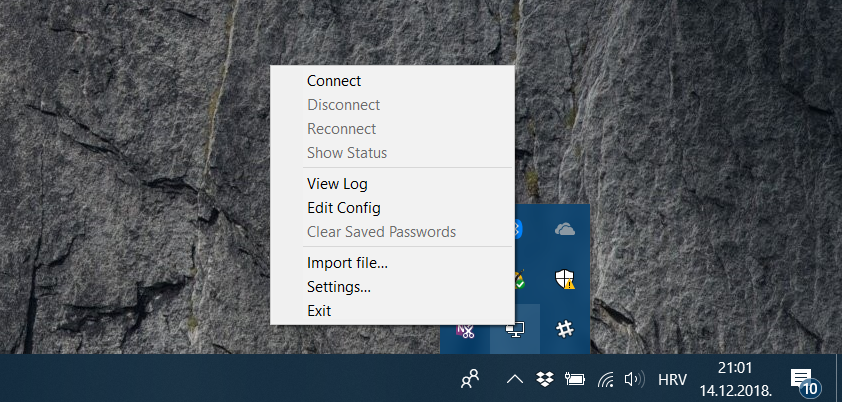
\includegraphics[width=0.7\linewidth]{slike/OpenVPN/win-open-vpn-2}
	\caption[Uvoz klijentske konfiguracije na Windowsima]{Uvoz klijentske konfiguracije na Windowsima}
	\label{fig:win-open-vpn-2}
\end{figure}
Desni klik na nju i odaberite Import file. Nakon toga navigirajte do mjesta gdje ste spremili client1.ovpn i odaberite datoteku. Zadnji korak je stisnuti na opciju Connect. Nakon toga će se pokrenuti proces spajanja i ako je sve prošlo uredu bit će te spojeni na vaš VPN poslužitelj i bit će vam dodijeljena nova IP adresa.

\bigbreak
\paragraph*{Instalacija na mobilnim uređajima}
\hfill \smallbreak
Instalacija na Android i iOS sustavima je gotovo identična. Ovdje će biti opisano spajanje na Android 8.1 operacijskom sustavu.
\begin{figure}[h]
	\centering
	\begin{subfigure}{0.49\textwidth}
		\centering
		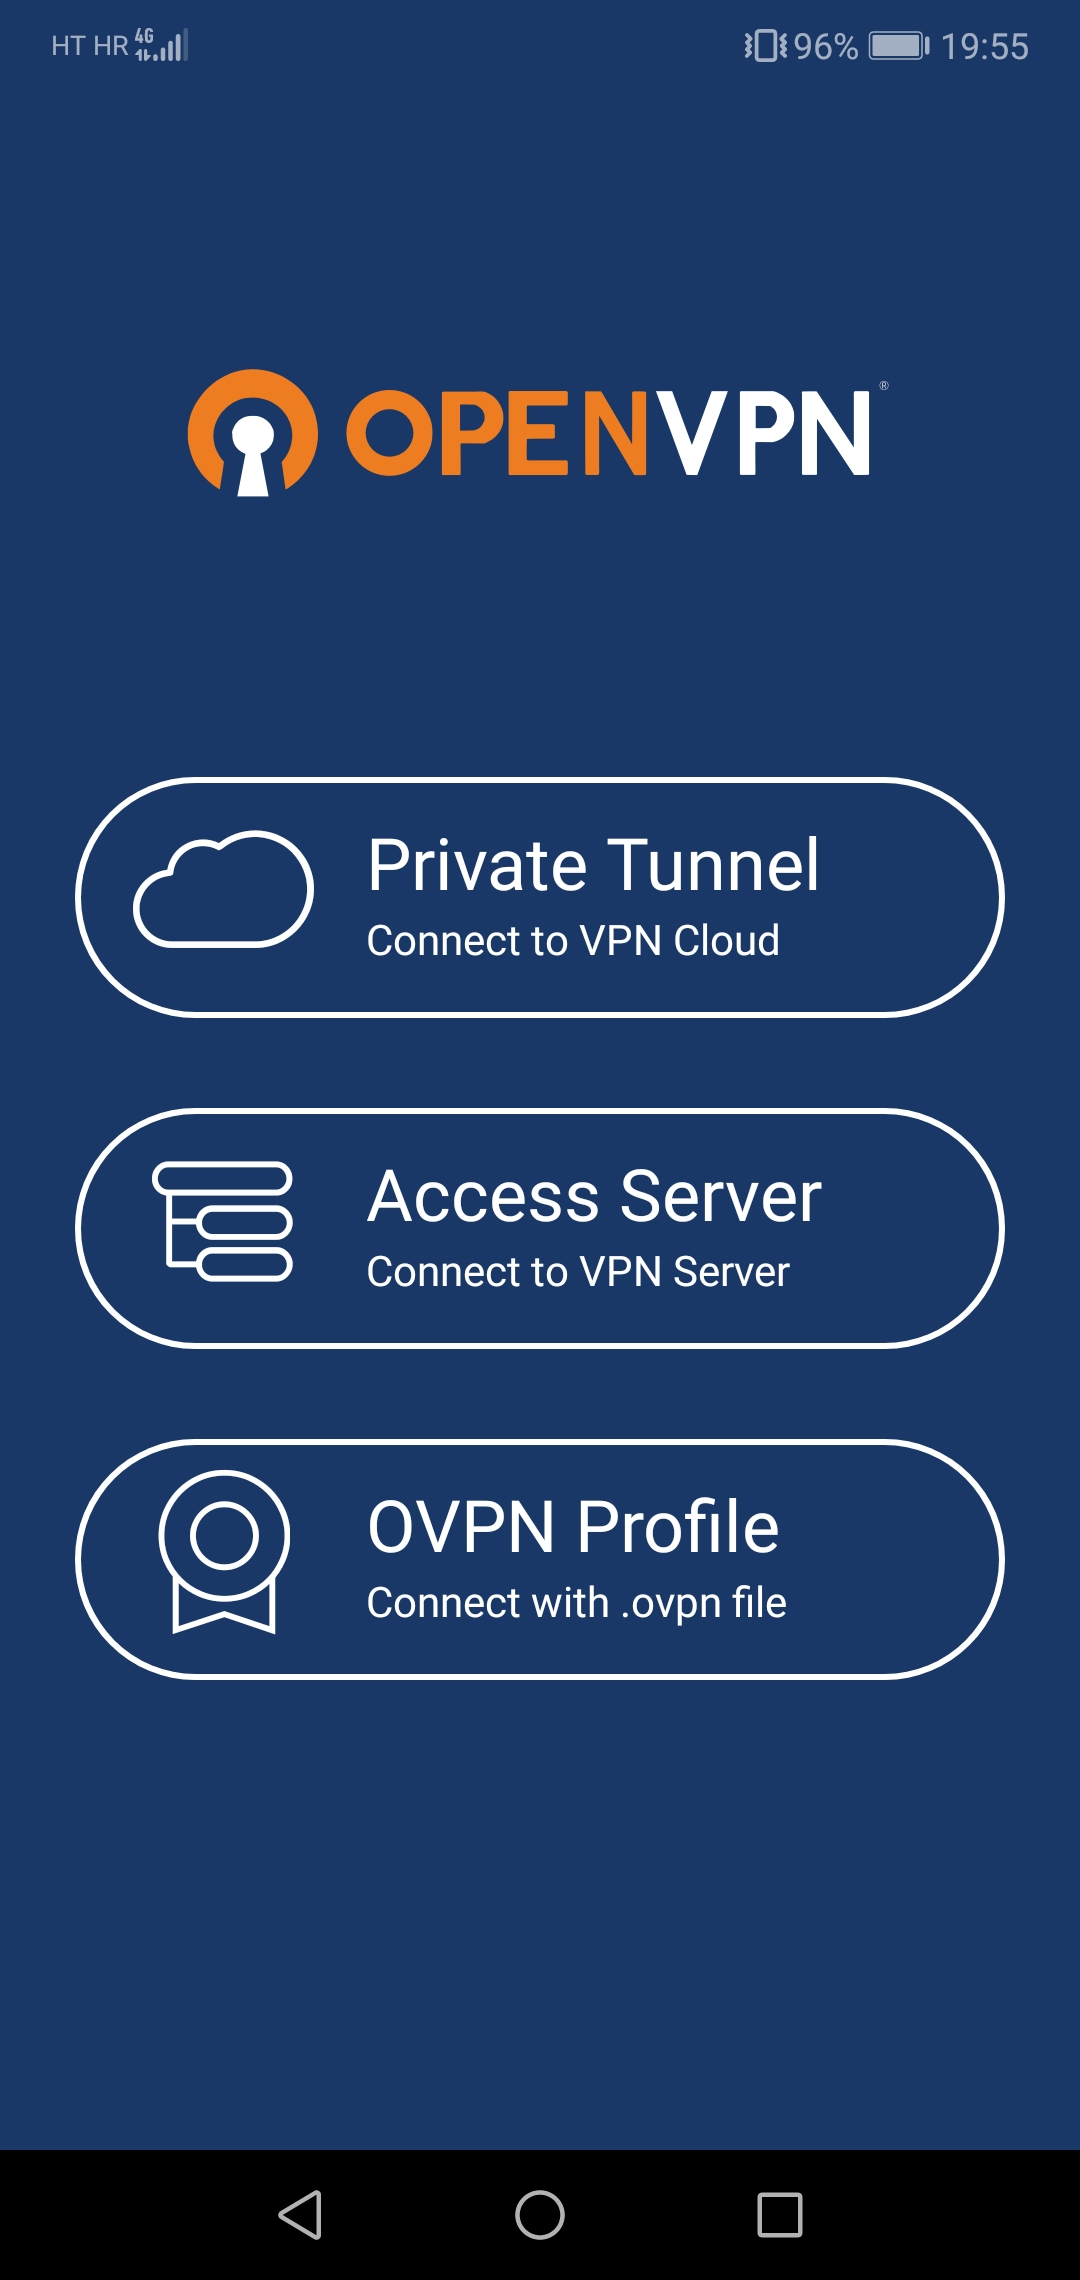
\includegraphics[width = 0.5\textwidth]{slike/OpenVPN/Screenshot_20181214-195518}
		\caption{Početni ekran OpenVPN aplikacije}
		\label{fig:screenshot20181214-195518}
	\end{subfigure}
	\begin{subfigure}{0.49\textwidth}
		\centering
		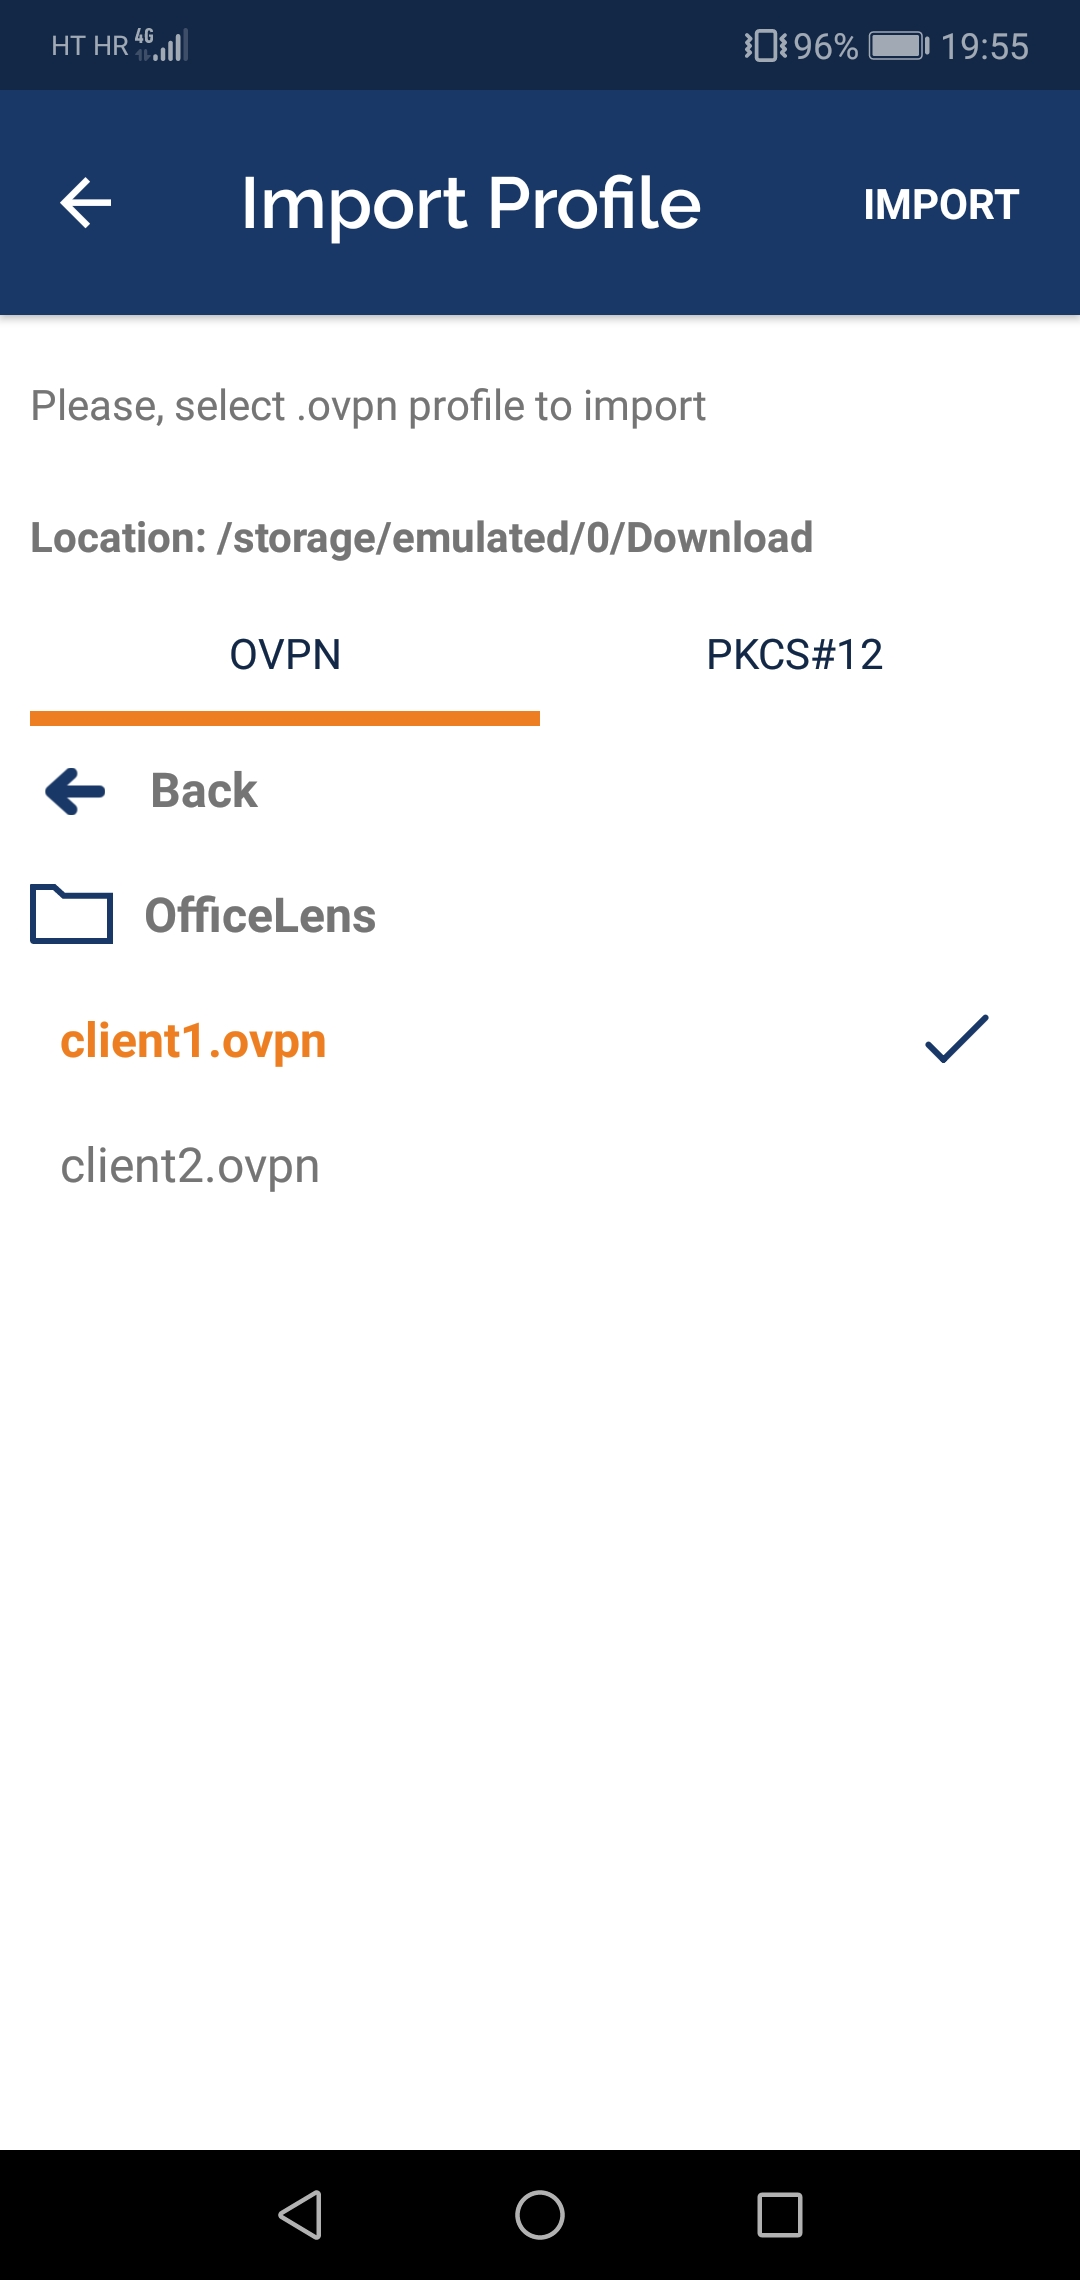
\includegraphics[width = 0.5\textwidth]{slike/OpenVPN/Screenshot_20181214-195554}
		\caption{Odabir klijentske konfiguracije}
		\label{fig:screenshot20181214-195554}
	\end{subfigure}
	\begin{subfigure}{0.49\textwidth}
		\centering
		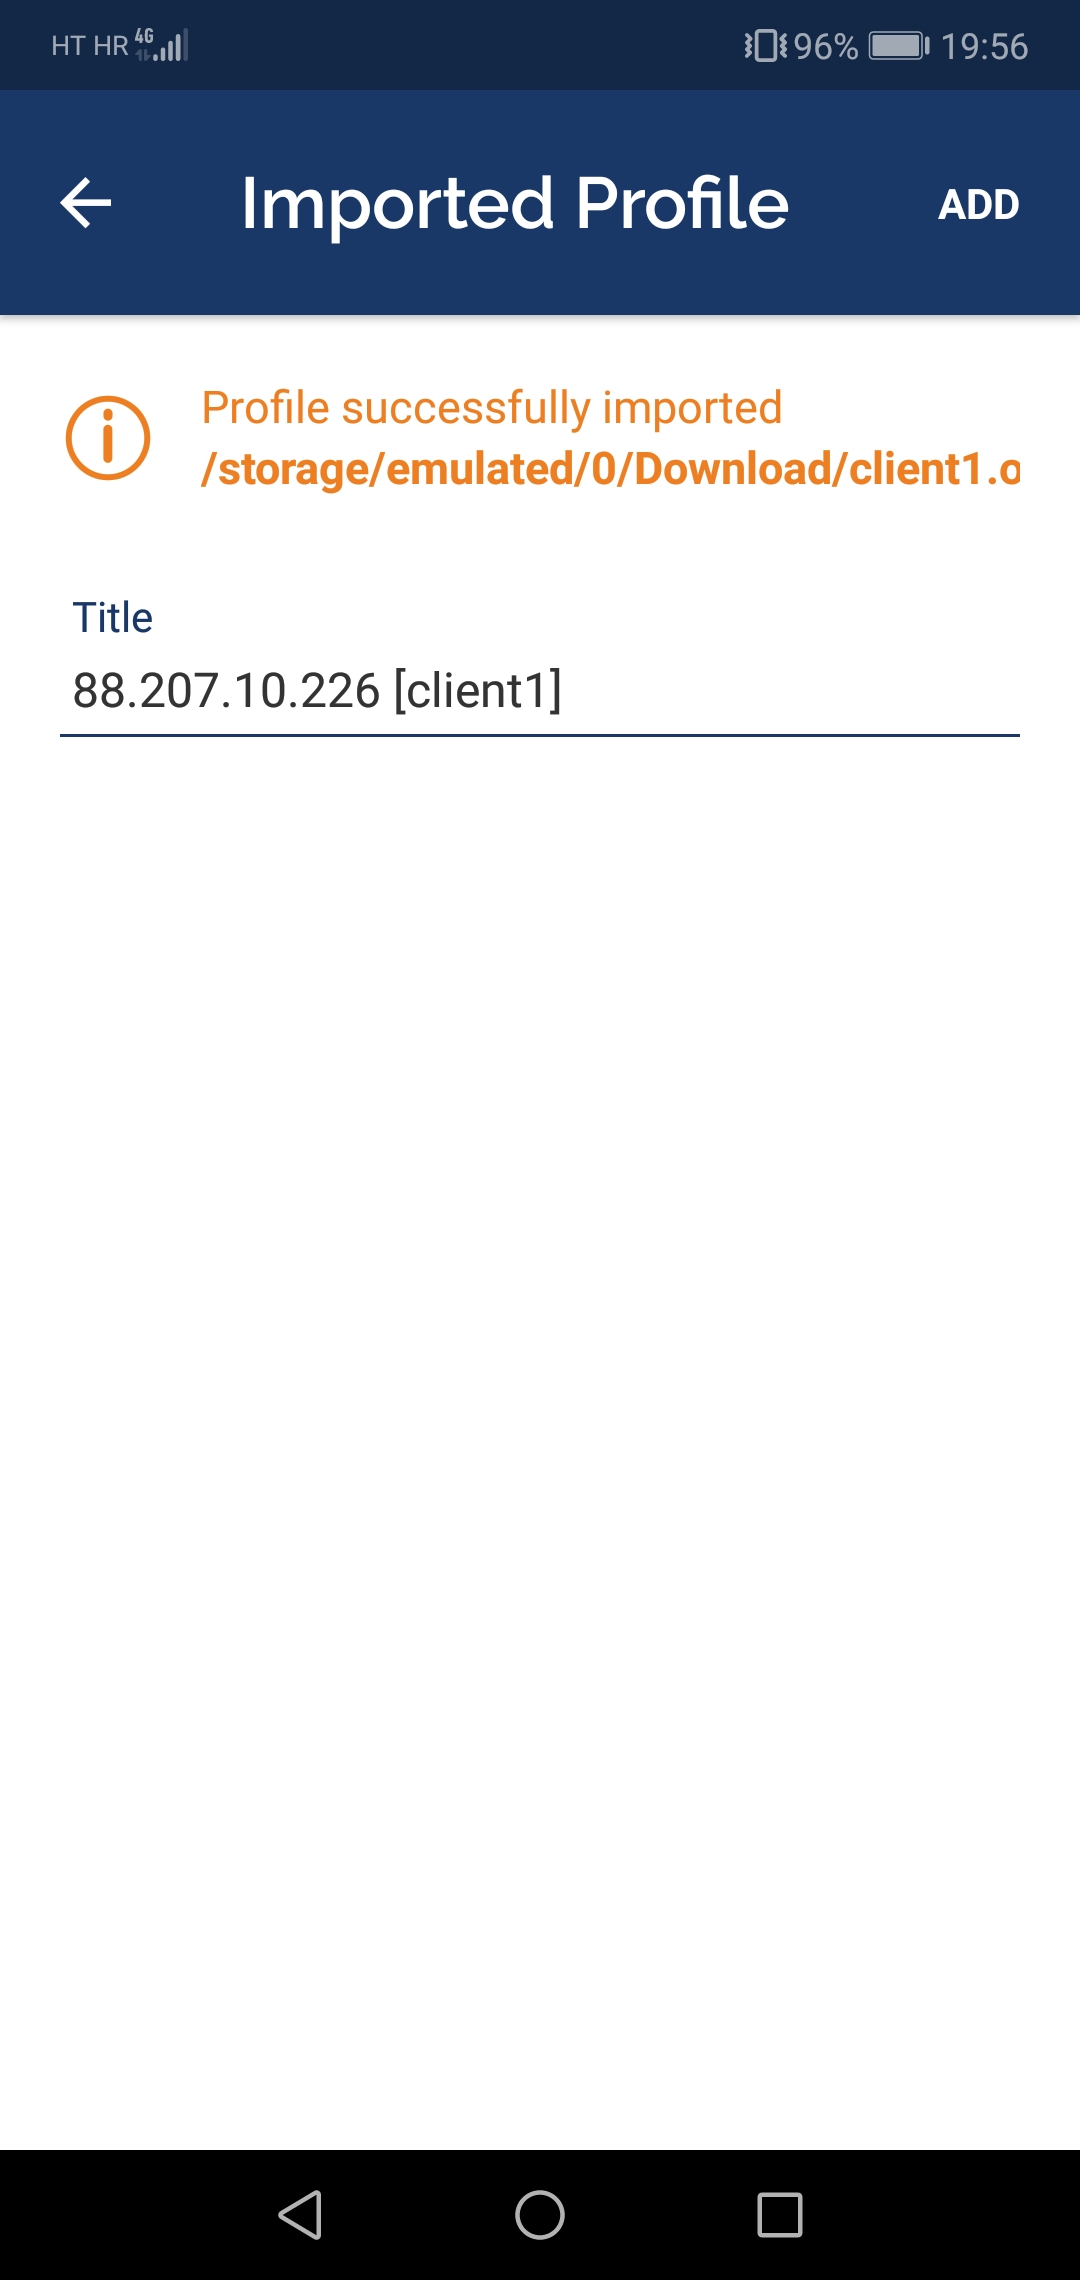
\includegraphics[width = 0.5\textwidth]{slike/OpenVPN/Screenshot_20181214-195602}
		\caption{Uspješno učitavanje profila}
		\label{fig:screenshot20181214-195602}
	\end{subfigure}
	\begin{subfigure}{0.49\textwidth}
		\centering
		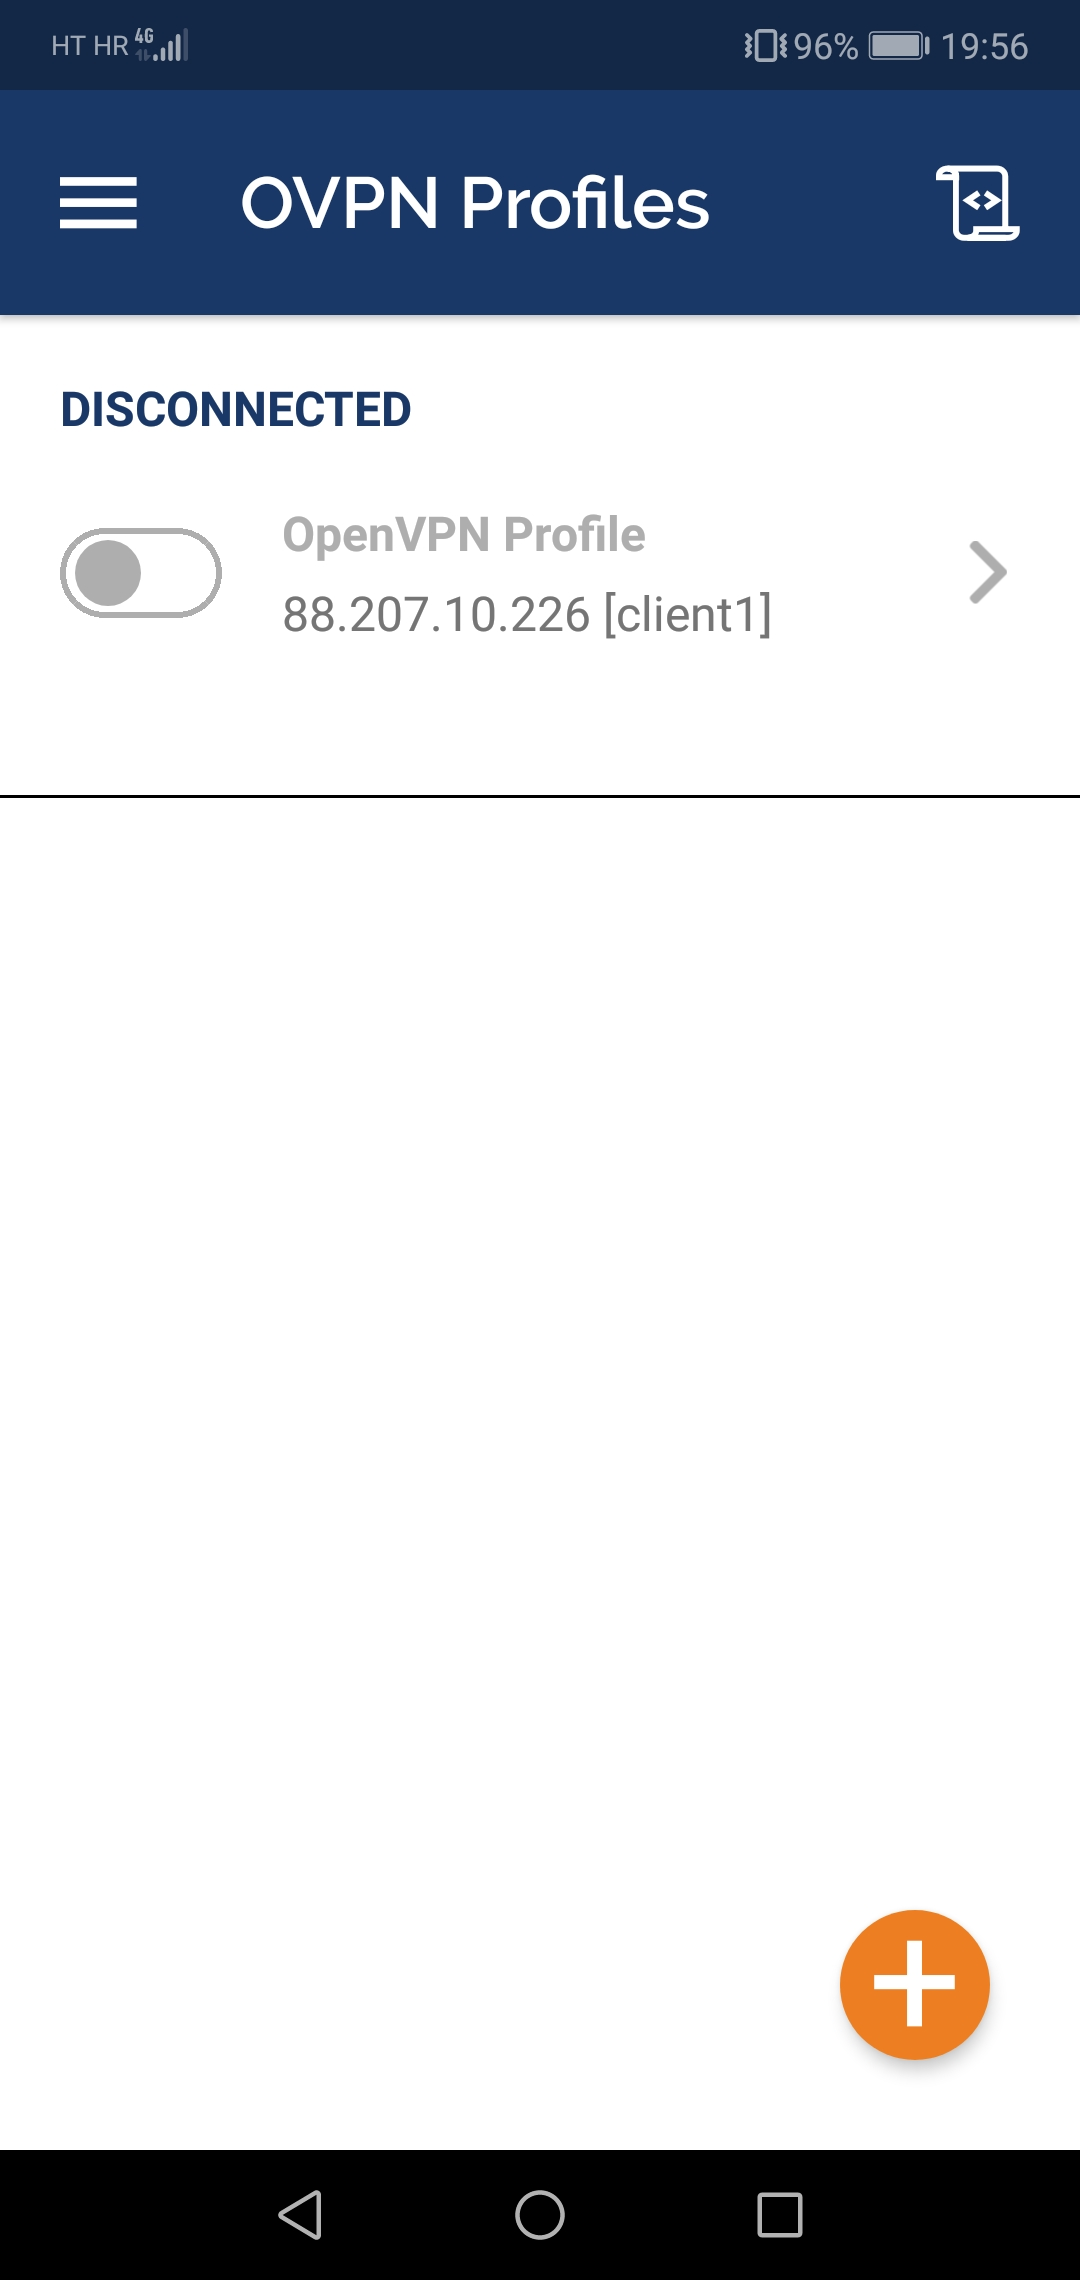
\includegraphics[width = 0.5\textwidth]{slike/OpenVPN/Screenshot_20181214-195614}
		\caption{Profil je uspješno dodan}
		\label{fig:screenshot20181214-195614}
	\end{subfigure}
	\caption{OpenVPN aplikacija}
	\label{fig:combined}
\end{figure}
\\Skinite aplikaciju OpenVPN i otvorite ju, bit će vam prikazan početni ekran kao na slici \ref{fig:screenshot20181214-195518}. Odaberite opciju spajanja preko OVPN profila. Profil bi već sada trebao biti dostupan ako ste ga skinuli s interneta, a ako niste onda navigirajte do njega. Odaberite profil client1.ovpn kao što je prikazano na slici \ref{fig:screenshot20181214-195554}.
Nakon toga dobit će te poruku o uspješnom učitavanju profila (slika: \ref{fig:screenshot20181214-195602} ). Stisnite na opciju ADD u gornjem desnom kutu. I na kraju se povežite s VPN poslužiteljem pritiskajući na sivi gumb (slika: \ref{fig:screenshot20181214-195614}). 


